\subsection{Exogenous IFIT2-FLAG Localisation in the Context of RSV pIBs and IBs} \label{subsec:Exogenous IFIT2-FLAG Localisation in the Context of RSV pIBs and IBs}
\subsubsection{IFIT2-FLAG in a Simplified System of pseudo-IBs} \label{IFIT2-FLAG in a Simplified System of pseudo-IBs}
Monkey cells transfected with human RSV N and P, along with human IFIT2-FLAG show concentration within the pIB structures as well as the pIB filamentous network. In this experiment we are detecting both human and monkey IFIT2, however we can see a huge difference in IFIT2 expression between some cells (bottom panel; cells in the periphery of the picture), suggesting that what we are mainly detecting is the overexpressed human IFIT2-FLAG.

\begin{figure}
    \begin{subfigure}{0.495\textwidth}
        \caption{}
        \includegraphics[width=1\linewidth]{09. Chapter 4/Figs/03. IFIT2-FLAG/01. IFIT2A/01. bar_i2a_hnhp.pdf} 
    \end{subfigure}
    \begin{subfigure}{0.495\textwidth}
        \caption{}
        \includegraphics[width=1\linewidth]{09. Chapter 4/Figs/03. IFIT2-FLAG/01. IFIT2A/02. box_i2a_hnhp.pdf}
    \end{subfigure}
    \caption[Observed Phenotypes of Exogenous Human IFIT2 in the Context of hRSV Pseudo Inclusion Bodies in VERO Cell Line, as Detected by IFIT2A Antibody.]{\textbf{Observed Phenotypes of Exogenous Human IFIT2 in the Context of hRSV Pseudo Inclusion Bodies in VERO Cell Line, as Detected by IFIT2A Antibody.} Vero cells were transfected with hRSV N and P, along with human IFIT2-FLAG containing plasmids using TransIT-X2 and were fixed after 24 hours. Cells were labeled with anti-RSV N and anti-IFIT2A antibodies and imaged on confocal microscope. Panel (a) shows percentual proportions of observed phenotypes between hRSV pseudo inclusion bodies and exogenous human IFIT2 (56 observations), with the red dotted line denoting the 5\% threshold, marking phenotypes considered relevant above this limit. Panel (b) shows the IB area in \(\mu m^2\) per observed relevant phenotype.}
    \label{fig:Observed Phenotypes of Exogenous Human IFIT2 in the Context of hRSV Pseudo Inclusion Bodies in VERO Cell Line, as Detected by IFIT2A Antibody}
\end{figure}

\begin{figure}
    \centering
    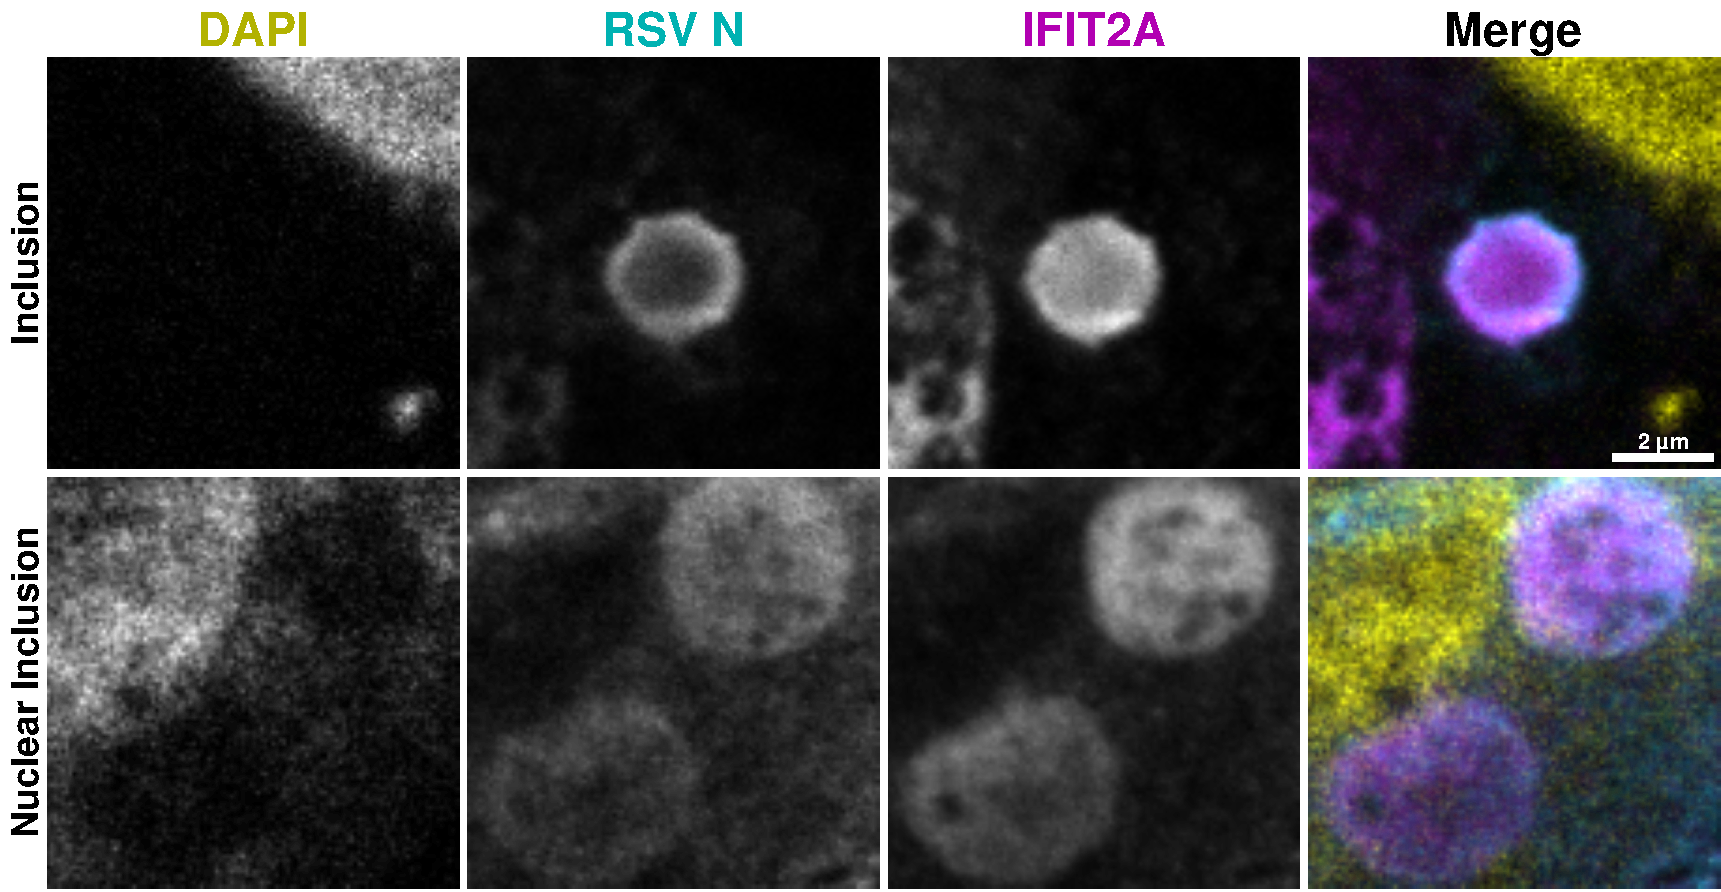
\includegraphics[width=1\linewidth]{09. Chapter 4/Figs/03. IFIT2-FLAG/01. IFIT2A/03. i2a-hi2f-hnhp.pdf}
    \caption[Representative Images of Observed Phenotypes of Exogenous Human IFIT2 in the Context of hRSV Pseudo Inclusion Bodies in VERO Cell Line, as Detected by IFIT2A Antibody.]{\textbf{Representative Images of Observed Phenotypes of Exogenous Human IFIT2 in the Context of hRSV Pseudo Inclusion Bodies in VERO Cell Line, as Detected by IFIT2A Antibody.} Vero cells were transfected with hRSV N and P, along with human IFIT2-FLAG containing plasmids using TransIT-X2 and were fixed after 24 hours. Cellular nuclei were stained with DAPI (yellow), and cells were double-labeled with anti-RSV N (cyan) and anti-IFIT2A (magenta) antibodies. This figure showcases representative examples of relevant phenotypes in the interaction between exogenous human IFIT2 and hRSV pseudo inclusion bodies. These phenotypes are presented in descending order based on their percentage proportions. The scale bar indicates 2 \(\mu m\).}
    \label{fig:Representative Images of Observed Phenotypes of Exogenous Human IFIT2 in the Context of hRSV Pseudo Inclusion Bodies in VERO Cell Line, as Detected by IFIT2A Antibody}
\end{figure}

Monkey cells transfected with human RSV N and P, along with human IFIT2-FLAG show concentration within the pIB structures but show exclusion from the pIB filamentous network (or partial colocalsiation?). This suggest that the IFIT2B antibody can indeed detect IFIT2 but the overexpressed IFIT2 observed between the inclusion and the one interacting with the filamentous network is somehow different (epitope masking?).

\begin{figure}
    \begin{subfigure}{0.495\textwidth}
        \caption{}
        \includegraphics[width=1\linewidth]{09. Chapter 4/Figs/03. IFIT2-FLAG/02. IFIT2B/01. bar_i2b_hnhp.pdf}
    \end{subfigure}
    \begin{subfigure}{0.495\textwidth}
        \caption{}
        \includegraphics[width=1\linewidth]{09. Chapter 4/Figs/03. IFIT2-FLAG/02. IFIT2B/02. box_i2a_hnhp.pdf}
    \end{subfigure}
    \caption[Observed Phenotypes of Exogenous Human IFIT2 in the Context of hRSV Pseudo Inclusion Bodies in VERO Cell Line, as Detected by IFIT2B Antibody.]{\textbf{Observed Phenotypes of Exogenous Human IFIT2 in the Context of hRSV Pseudo Inclusion Bodies in VERO Cell Line, as Detected by IFIT2B Antibody.} Vero cells were transfected with hRSV N and P, along with human IFIT2-FLAG containing plasmids using TransIT-X2 and were fixed after 24 hours. Cells were labeled with anti-RSV N and anti-IFIT2B antibodies and imaged on confocal microscope. Panel (a) shows percentual proportions of observed phenotypes between hRSV pseudo inclusion bodies and exogenous human IFIT2 (44 observations), with the red dotted line denoting the 5\% threshold, marking phenotypes considered relevant above this limit. Panel (b) shows the IB area in \(\mu m^2\) per observed relevant phenotype.}
    \label{fig:Observed Phenotypes of Exogenous Human IFIT2 in the Context of hRSV Pseudo Inclusion Bodies in VERO Cell Line, as Detected by IFIT2B Antibody}
\end{figure}

\begin{figure}
    \centering
    \includegraphics[width=1\linewidth]{09. Chapter 4/Figs/03. IFIT2-FLAG/02. IFIT2B/03. i2b-hi2f-hnhp.pdf}
    \caption[Representative Images of Observed Phenotypes of Exogenous Human IFIT2 in the Context of hRSV Pseudo Inclusion Bodies in VERO Cell Line, as Detected by IFIT2B Antibody.]{\textbf{Representative Images of Observed Phenotypes of Exogenous Human IFIT2 in the Context of hRSV Pseudo Inclusion Bodies in VERO Cell Line, as Detected by IFIT2B Antibody.} Vero cells were transfected with hRSV N and P, along with human IFIT2-FLAG containing plasmids using TransIT-X2 and were fixed after 24 hours. Cellular nuclei were stained with DAPI (yellow), and cells were double-labeled with anti-RSV N (cyan) and anti-IFIT2B (magenta) antibodies. This figure showcases representative examples of relevant phenotypes in the interaction between exogenous human IFIT2 and hRSV pseudo inclusion bodies. These phenotypes are presented in descending order based on their percentage proportions. The scale bar indicates 2 \(\mu m\).}
    \label{fig:Representative Images of Observed Phenotypes of Exogenous Human IFIT2 in the Context of hRSV Pseudo Inclusion Bodies in VERO Cell Line, as Detected by IFIT2B Antibody}
\end{figure}

Exogenously expressed human IFIT2 colocalises with the pIB associated filamentous net (top panel). It also forms inclusion inside the human pIB structures. This data is consistent with what we observed with IFIT2A antibody. IFIT2 also seems to occasionally form aggregates/spots (highlighted by arrows). These could be functional or just aggregates caused by overexpression, we do not know.

\begin{figure}
    \begin{subfigure}{0.495\textwidth}
        \caption{}
        \includegraphics[width=1\linewidth]{09. Chapter 4/Figs/03. IFIT2-FLAG/03. IFIT2F/01. pIB/01. bar_hi2f_hnhp.pdf}
    \end{subfigure}
    \begin{subfigure}{0.495\textwidth}
        \caption{}
        \includegraphics[width=1\linewidth]{09. Chapter 4/Figs/03. IFIT2-FLAG/03. IFIT2F/01. pIB/02. box_hi2f_hnhp.pdf}
    \end{subfigure}
    \caption[Observed Phenotypes of Exogenous Human IFIT2 in the Context of hRSV Pseudo Inclusion Bodies in VERO Cell Line, as Detected by FLAG Antibody.]{\textbf{Observed Phenotypes of Exogenous Human IFIT2 in the Context of hRSV Pseudo Inclusion Bodies in VERO Cell Line, as Detected by FLAG Antibody.} Vero cells were transfected with hRSV N and P, along with human IFIT2-FLAG containing plasmids using TransIT-X2 and were fixed after 24 hours. Cells were labeled with anti-RSV N and anti-FLAG antibodies and imaged on confocal microscope. Panel (a) shows percentual proportions of observed phenotypes between hRSV pseudo inclusion bodies and exogenous human IFIT2 (116 observations), with the red dotted line denoting the 5\% threshold, marking phenotypes considered relevant above this limit. Panel (b) shows the IB area in \(\mu m^2\) per observed relevant phenotype.}
    \label{fig:Observed Phenotypes of Exogenous Human IFIT2 in the Context of hRSV Pseudo Inclusion Bodies in VERO Cell Line, as Detected by FLAG Antibody}
\end{figure}

\begin{figure}
    \centering
    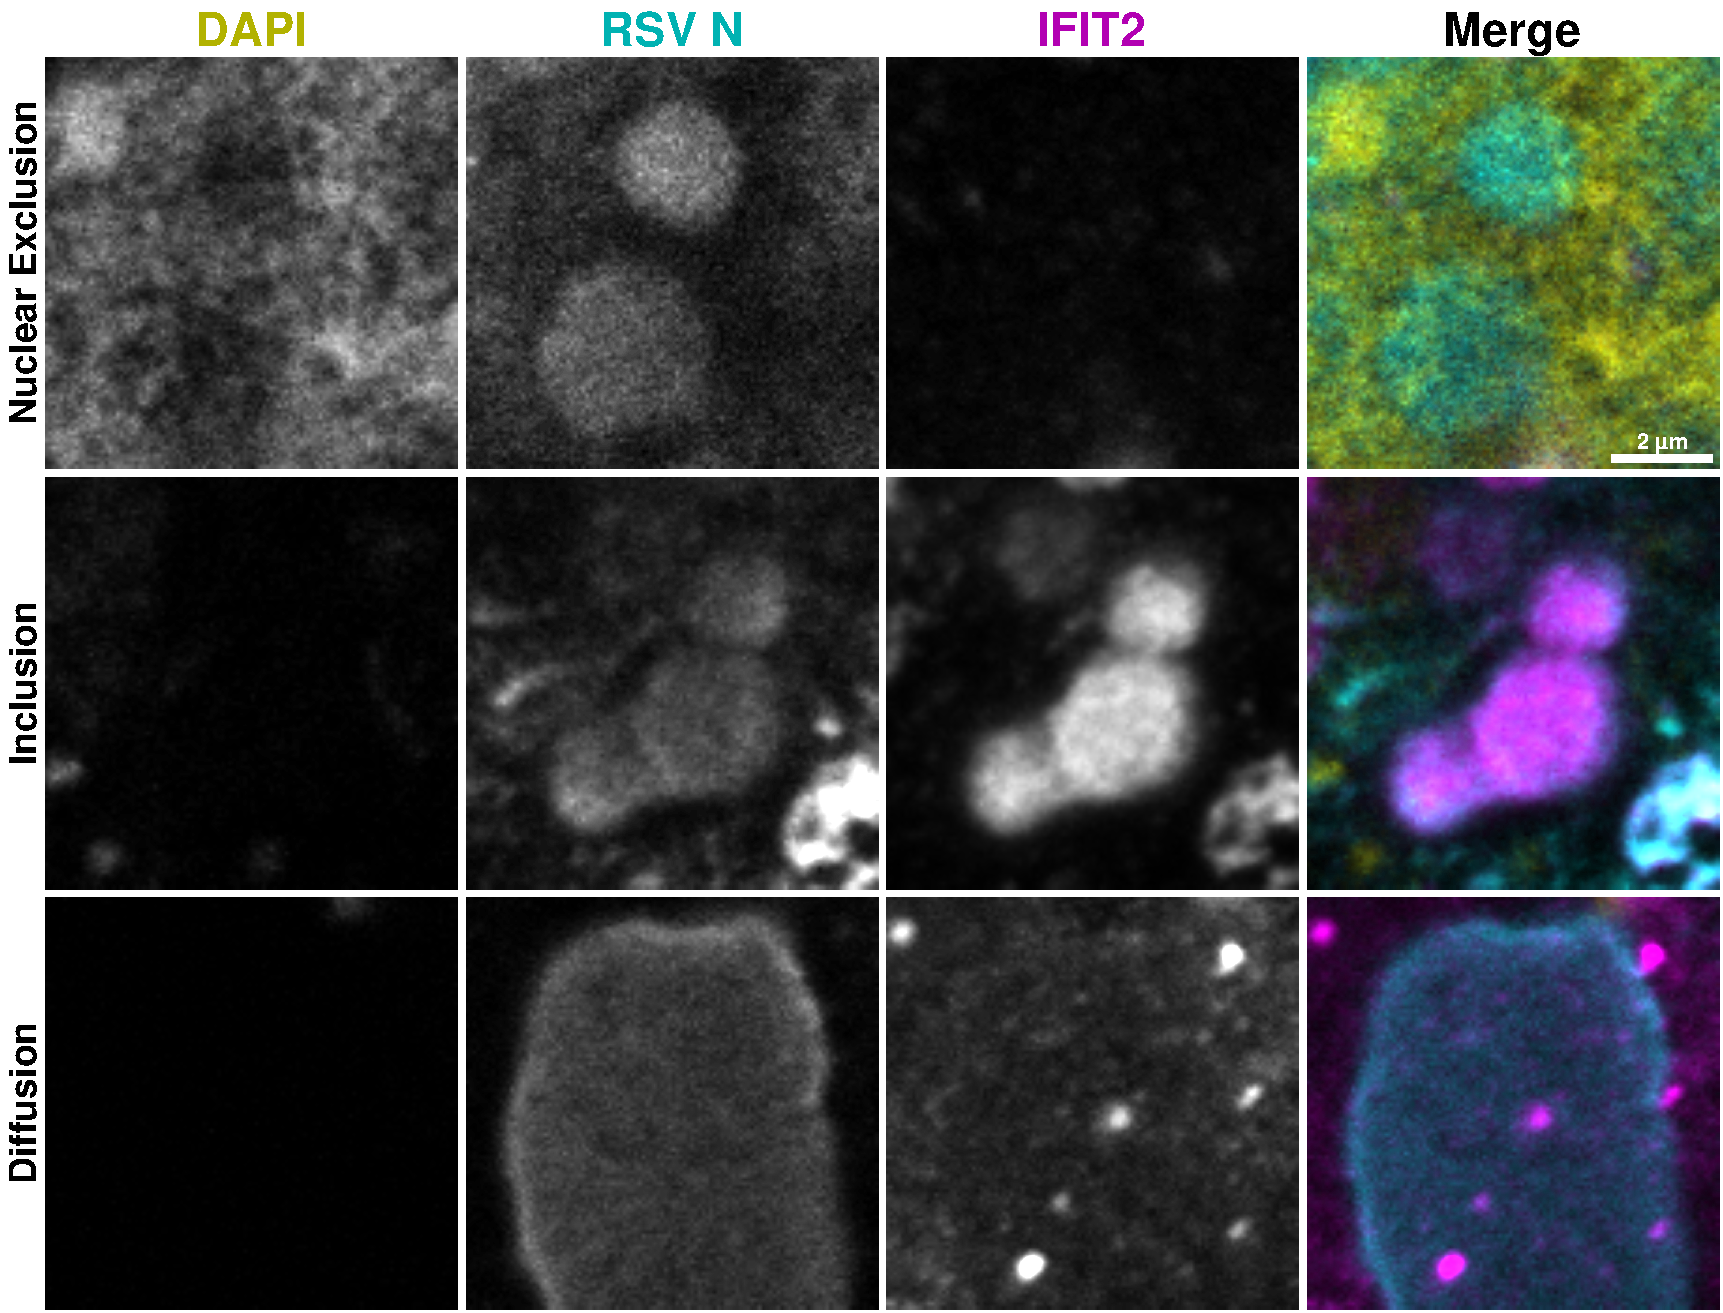
\includegraphics[width=1\linewidth]{09. Chapter 4/Figs/03. IFIT2-FLAG/03. IFIT2F/01. pIB/03. hi2f-hnhp.pdf}
    \caption[Representative Images of Observed Phenotypes of Exogenous Human IFIT2 in the Context of hRSV Pseudo Inclusion Bodies in VERO Cell Line, as Detected by FLAG Antibody.]{\textbf{Representative Images of Observed Phenotypes of Exogenous Human IFIT2 in the Context of hRSV Pseudo Inclusion Bodies in VERO Cell Line, as Detected by FLAG Antibody.} Vero cells were transfected with hRSV N and P, along with human IFIT2-FLAG containing plasmids using TransIT-X2 and were fixed after 24 hours. Cellular nuclei were stained with DAPI (yellow), and cells were double-labeled with anti-RSV N (cyan) and anti-FLAG (magenta) antibodies. This figure showcases representative examples of relevant phenotypes in the interaction between exogenous human IFIT2 and hRSV pseudo inclusion bodies. These phenotypes are presented in descending order based on their percentage proportions. The scale bar indicates 2 \(\mu m\).}
    \label{fig:Representative Images of Observed Phenotypes of Exogenous Human IFIT2 in the Context of hRSV Pseudo Inclusion Bodies in VERO Cell Line, as Detected by FLAG Antibody}
\end{figure}

Exogenous bovine IFIT2 colocalises with the edge of human pIB structures. This is unusual as human IFIT2 data suggest inclusions with regards to pIBs.  

\begin{figure}
    \begin{subfigure}{0.495\textwidth}
        \caption{}
        \includegraphics[width=1\linewidth]{09. Chapter 4/Figs/03. IFIT2-FLAG/03. IFIT2F/01. pIB/04. bar_bi2f_hnhp.pdf} 
    \end{subfigure}
    \begin{subfigure}{0.495\textwidth}
        \caption{}
        \includegraphics[width=1\linewidth]{09. Chapter 4/Figs/03. IFIT2-FLAG/03. IFIT2F/01. pIB/05. box_bi2f_hnhp.pdf}
    \end{subfigure}
    \caption[Observed Phenotypes of Exogenous Bovine IFIT2 in the Context of hRSV Pseudo Inclusion Bodies in VERO Cell Line, as Detected by FLAG Antibody.]{\textbf{Observed Phenotypes of Exogenous Bovine IFIT2 in the Context of hRSV Pseudo Inclusion Bodies in VERO Cell Line, as Detected by FLAG Antibody.} Vero cells were transfected with hRSV N and P, along with bovine IFIT2-FLAG containing plasmids using TransIT-X2 and were fixed after 24 hours. Cells were labeled with anti-RSV N and anti-FLAG antibodies and imaged on confocal microscope. Panel (a) shows percentual proportions of observed phenotypes between hRSV pseudo inclusion bodies and exogenous bovine IFIT2 (142 observations), with the red dotted line denoting the 5\% threshold, marking phenotypes considered relevant above this limit. Panel (b) shows the IB area in \(\mu m^2\) per observed relevant phenotype.}
    \label{fig:Observed Phenotypes of Exogenous Bovine IFIT2 in the Context of hRSV Pseudo Inclusion Bodies in VERO Cell Line, as Detected by FLAG Antibody}
\end{figure}

\begin{figure}
    \centering
    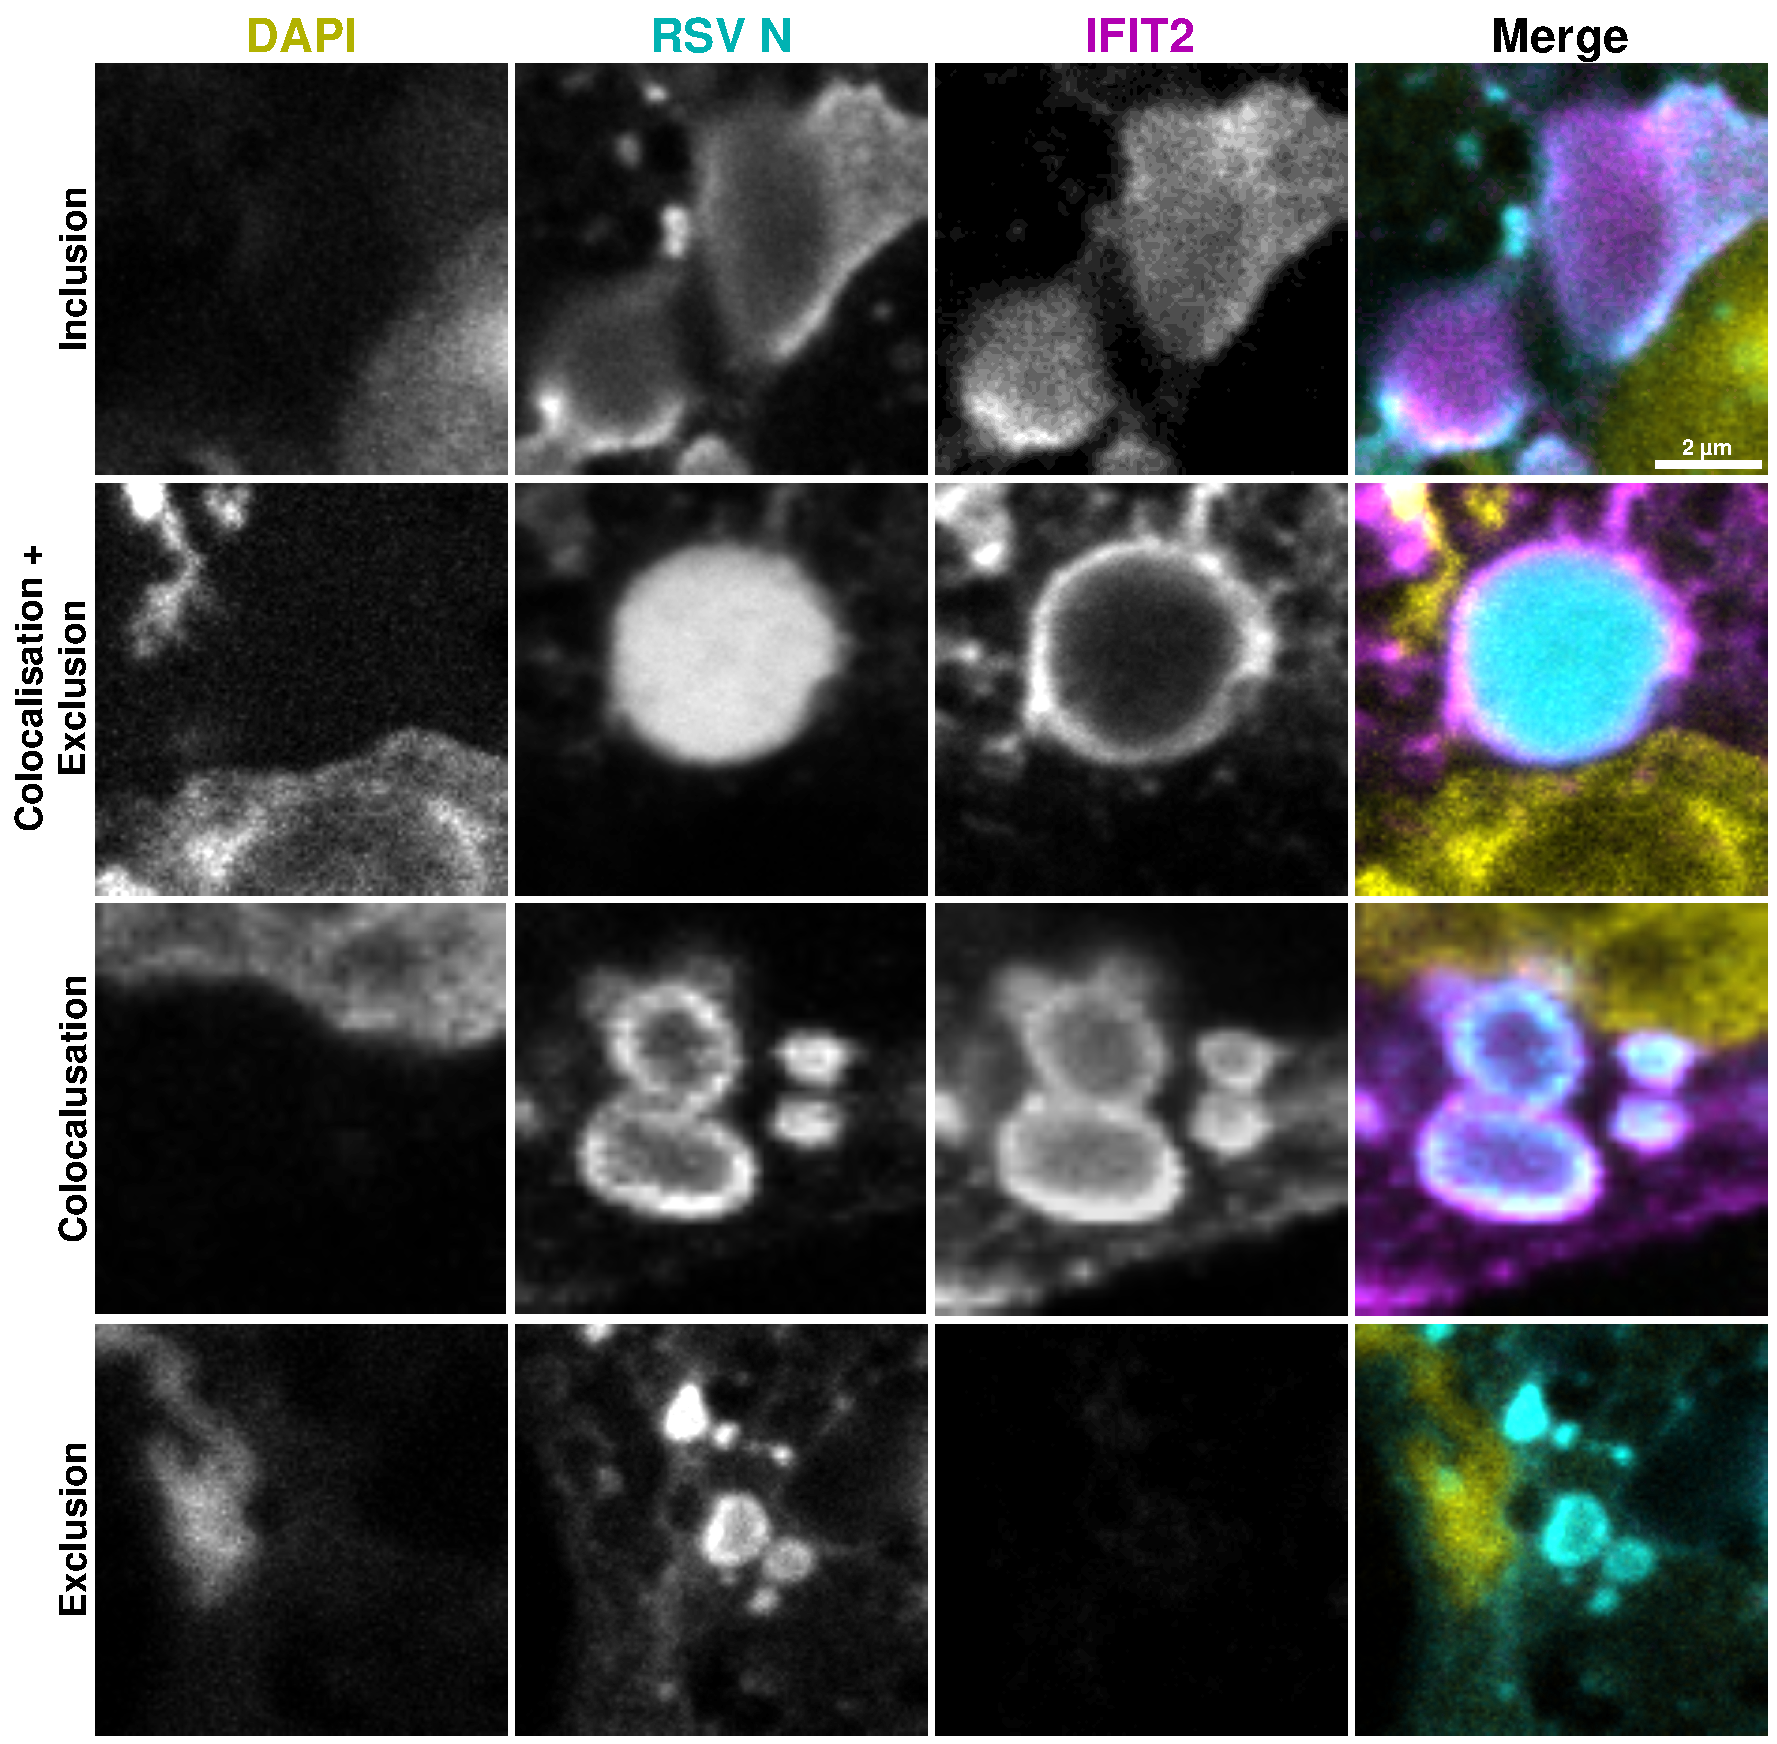
\includegraphics[width=1\linewidth]{09. Chapter 4/Figs/03. IFIT2-FLAG/03. IFIT2F/01. pIB/06. bi2f-hnhp.pdf}
    \caption[Representative Images of Observed Phenotypes of Exogenous Bovine IFIT2 in the Context of hRSV Pseudo Inclusion Bodies in VERO Cell Line, as Detected by FLAG Antibody.]{\textbf{Representative Images of Observed Phenotypes of Exogenous Bovine IFIT2 in the Context of hRSV Pseudo Inclusion Bodies in VERO Cell Line, as Detected by FLAG Antibody.} Vero cells were transfected with hRSV N and P, along with bovine IFIT2-FLAG containing plasmids using TransIT-X2 and were fixed after 24 hours. Cellular nuclei were stained with DAPI (yellow), and cells were double-labeled with anti-RSV N (cyan) and anti-FLAG (magenta) antibodies. This figure showcases representative examples of relevant phenotypes in the interaction between exogenous bovine IFIT2 and hRSV pseudo inclusion bodies. These phenotypes are presented in descending order based on their percentage proportions. The scale bar indicates 2 \(\mu m\).}
    \label{fig:Representative Images of Observed Phenotypes of Exogenous Bovine IFIT2 in the Context of hRSV Pseudo Inclusion Bodies in VERO Cell Line, as Detected by FLAG Antibody}
\end{figure}

\begin{figure}
    \begin{subfigure}{0.495\textwidth}
        \caption{}
        \includegraphics[width=1\linewidth]{09. Chapter 4/Figs/03. IFIT2-FLAG/03. IFIT2F/01. pIB/07. bar_bi2f_bnbp.pdf} 
    \end{subfigure}
    \begin{subfigure}{0.495\textwidth}
        \caption{}
        \includegraphics[width=1\linewidth]{09. Chapter 4/Figs/03. IFIT2-FLAG/03. IFIT2F/01. pIB/08. box_bi2f_bnbp.pdf}
    \end{subfigure}
    \caption[Observed Phenotypes of Exogenous Bovine IFIT2 in the Context of bRSV Pseudo Inclusion Bodies in VERO Cell Line, as Detected by FLAG Antibody.]{\textbf{Observed Phenotypes of Exogenous Bovine IFIT2 in the Context of bRSV Pseudo Inclusion Bodies in VERO Cell Line, as Detected by FLAG Antibody.} Vero cells were transfected with bRSV N and P, along with bovine IFIT2-FLAG containing plasmids using TransIT-X2 and were fixed after 24 hours. Cells were labeled with anti-RSV N and anti-FLAG antibodies and imaged on confocal microscope. Panel (a) shows percentual proportions of observed phenotypes between bRSV pseudo inclusion bodies and exogenous bovine IFIT2 (22 observations), with the red dotted line denoting the 5\% threshold, marking phenotypes considered relevant above this limit. Panel (b) shows the IB area in \(\mu m^2\) per observed relevant phenotype.}
    \label{fig:Observed Phenotypes of Exogenous Bovine IFIT2 in the Context of bRSV Pseudo Inclusion Bodies in VERO Cell Line, as Detected by FLAG Antibody}
\end{figure}

\begin{figure}
    \centering
    \includegraphics[width=1\linewidth]{09. Chapter 4/Figs/03. IFIT2-FLAG/03. IFIT2F/01. pIB/09. bi2f-bnbp.pdf}
    \caption[Representative Images of Observed Phenotypes of Exogenous Bovine IFIT2 in the Context of bRSV Pseudo Inclusion Bodies in VERO Cell Line, as Detected by FLAG Antibody.]{\textbf{Representative Images of Observed Phenotypes of Exogenous Bovine IFIT2 in the Context of bRSV Pseudo Inclusion Bodies in VERO Cell Line, as Detected by FLAG Antibody.} Vero cells were transfected with bRSV N and P, along with bovine IFIT2-FLAG containing plasmids using TransIT-X2 and were fixed after 24 hours. Cellular nuclei were stained with DAPI (yellow), and cells were double-labeled with anti-RSV N (cyan) and anti-FLAG (magenta) antibodies. This figure showcases representative examples of relevant phenotypes in the interaction between exogenous bovine IFIT2 and bRSV pseudo inclusion bodies. These phenotypes are presented in descending order based on their percentage proportions. The scale bar indicates 2 \(\mu m\).}
    \label{fig:Representative Images of Observed Phenotypes of Exogenous Bovine IFIT2 in the Context of bRSV Pseudo Inclusion Bodies in VERO Cell Line, as Detected by FLAG Antibody}
\end{figure}

\subsubsection{Exogenous IFIT2-FLAG During RSV Infection} \label{Exogenous IFIT2-FLAG During RSV Infection}
Overexpressed human IFIT2 during hRSV infection shows several phenotypes (in this experiment). We see IFIT2 being excluded from the IB interior while being concentrated to the IB ring (top panel); IFIT2 forming concentrated inclusion inside the IB structure (2nd panel); IFIT2 being excluded from the IB interior but colocalising to the IB ring and forming spots inside of the IB (3rd panel); and IFIT2 being diffused evenly through the cytoplasm and the IB structure (last panel). The different phenotypes suggest that IBs are dynamic structures, and the localisation depends on factors we do not comprehend yet. 

\begin{figure}
    \begin{subfigure}{0.495\textwidth}
        \caption{}
        \includegraphics[width=1\linewidth]{09. Chapter 4/Figs/03. IFIT2-FLAG/03. IFIT2F/02. Infection Transfection/01. bar_hi2f_hrsv.pdf} 
    \end{subfigure}
    \begin{subfigure}{0.495\textwidth}
        \caption{}
        \includegraphics[width=1\linewidth]{09. Chapter 4/Figs/03. IFIT2-FLAG/03. IFIT2F/02. Infection Transfection/02. box_hi2f_hrsv.pdf}
    \end{subfigure}
    \caption[Observed Phenotypes of Exogenous hIFIT2 in the Context of hRSV Inclusion Bodies in VERO Cell Line.]{\textbf{Observed Phenotypes of Exogenous hIFIT2 in the Context of hRSV Inclusion Bodies in VERO Cell Line.} Vero cells were infected with human RSV at MOI 1. 24 HPI, the cells were transfected with hIFIT2-FLAG containing plasmids using TransIT-X2 and were fixed after further 24 hours. Cells were labeled with anti-RSV N and anti-FLAG antibodies and imaged on confocal microscope. Panel (a) shows percentual proportions of observed phenotypes between hRSV inclusion bodies and exogenous hIFIT2 (155 observations), with the red dotted line denoting the 5\% threshold, marking phenotypes considered relevant above this limit. Panel (b) shows the IB area in \(\mu m^2\) per observed relevant phenotype.}
    \label{fig:Observed Phenotypes of Exogenous hIFIT2 in the Context of hRSV Inclusion Bodies in VERO Cell Line}
\end{figure}

\begin{figure}
    \centering
    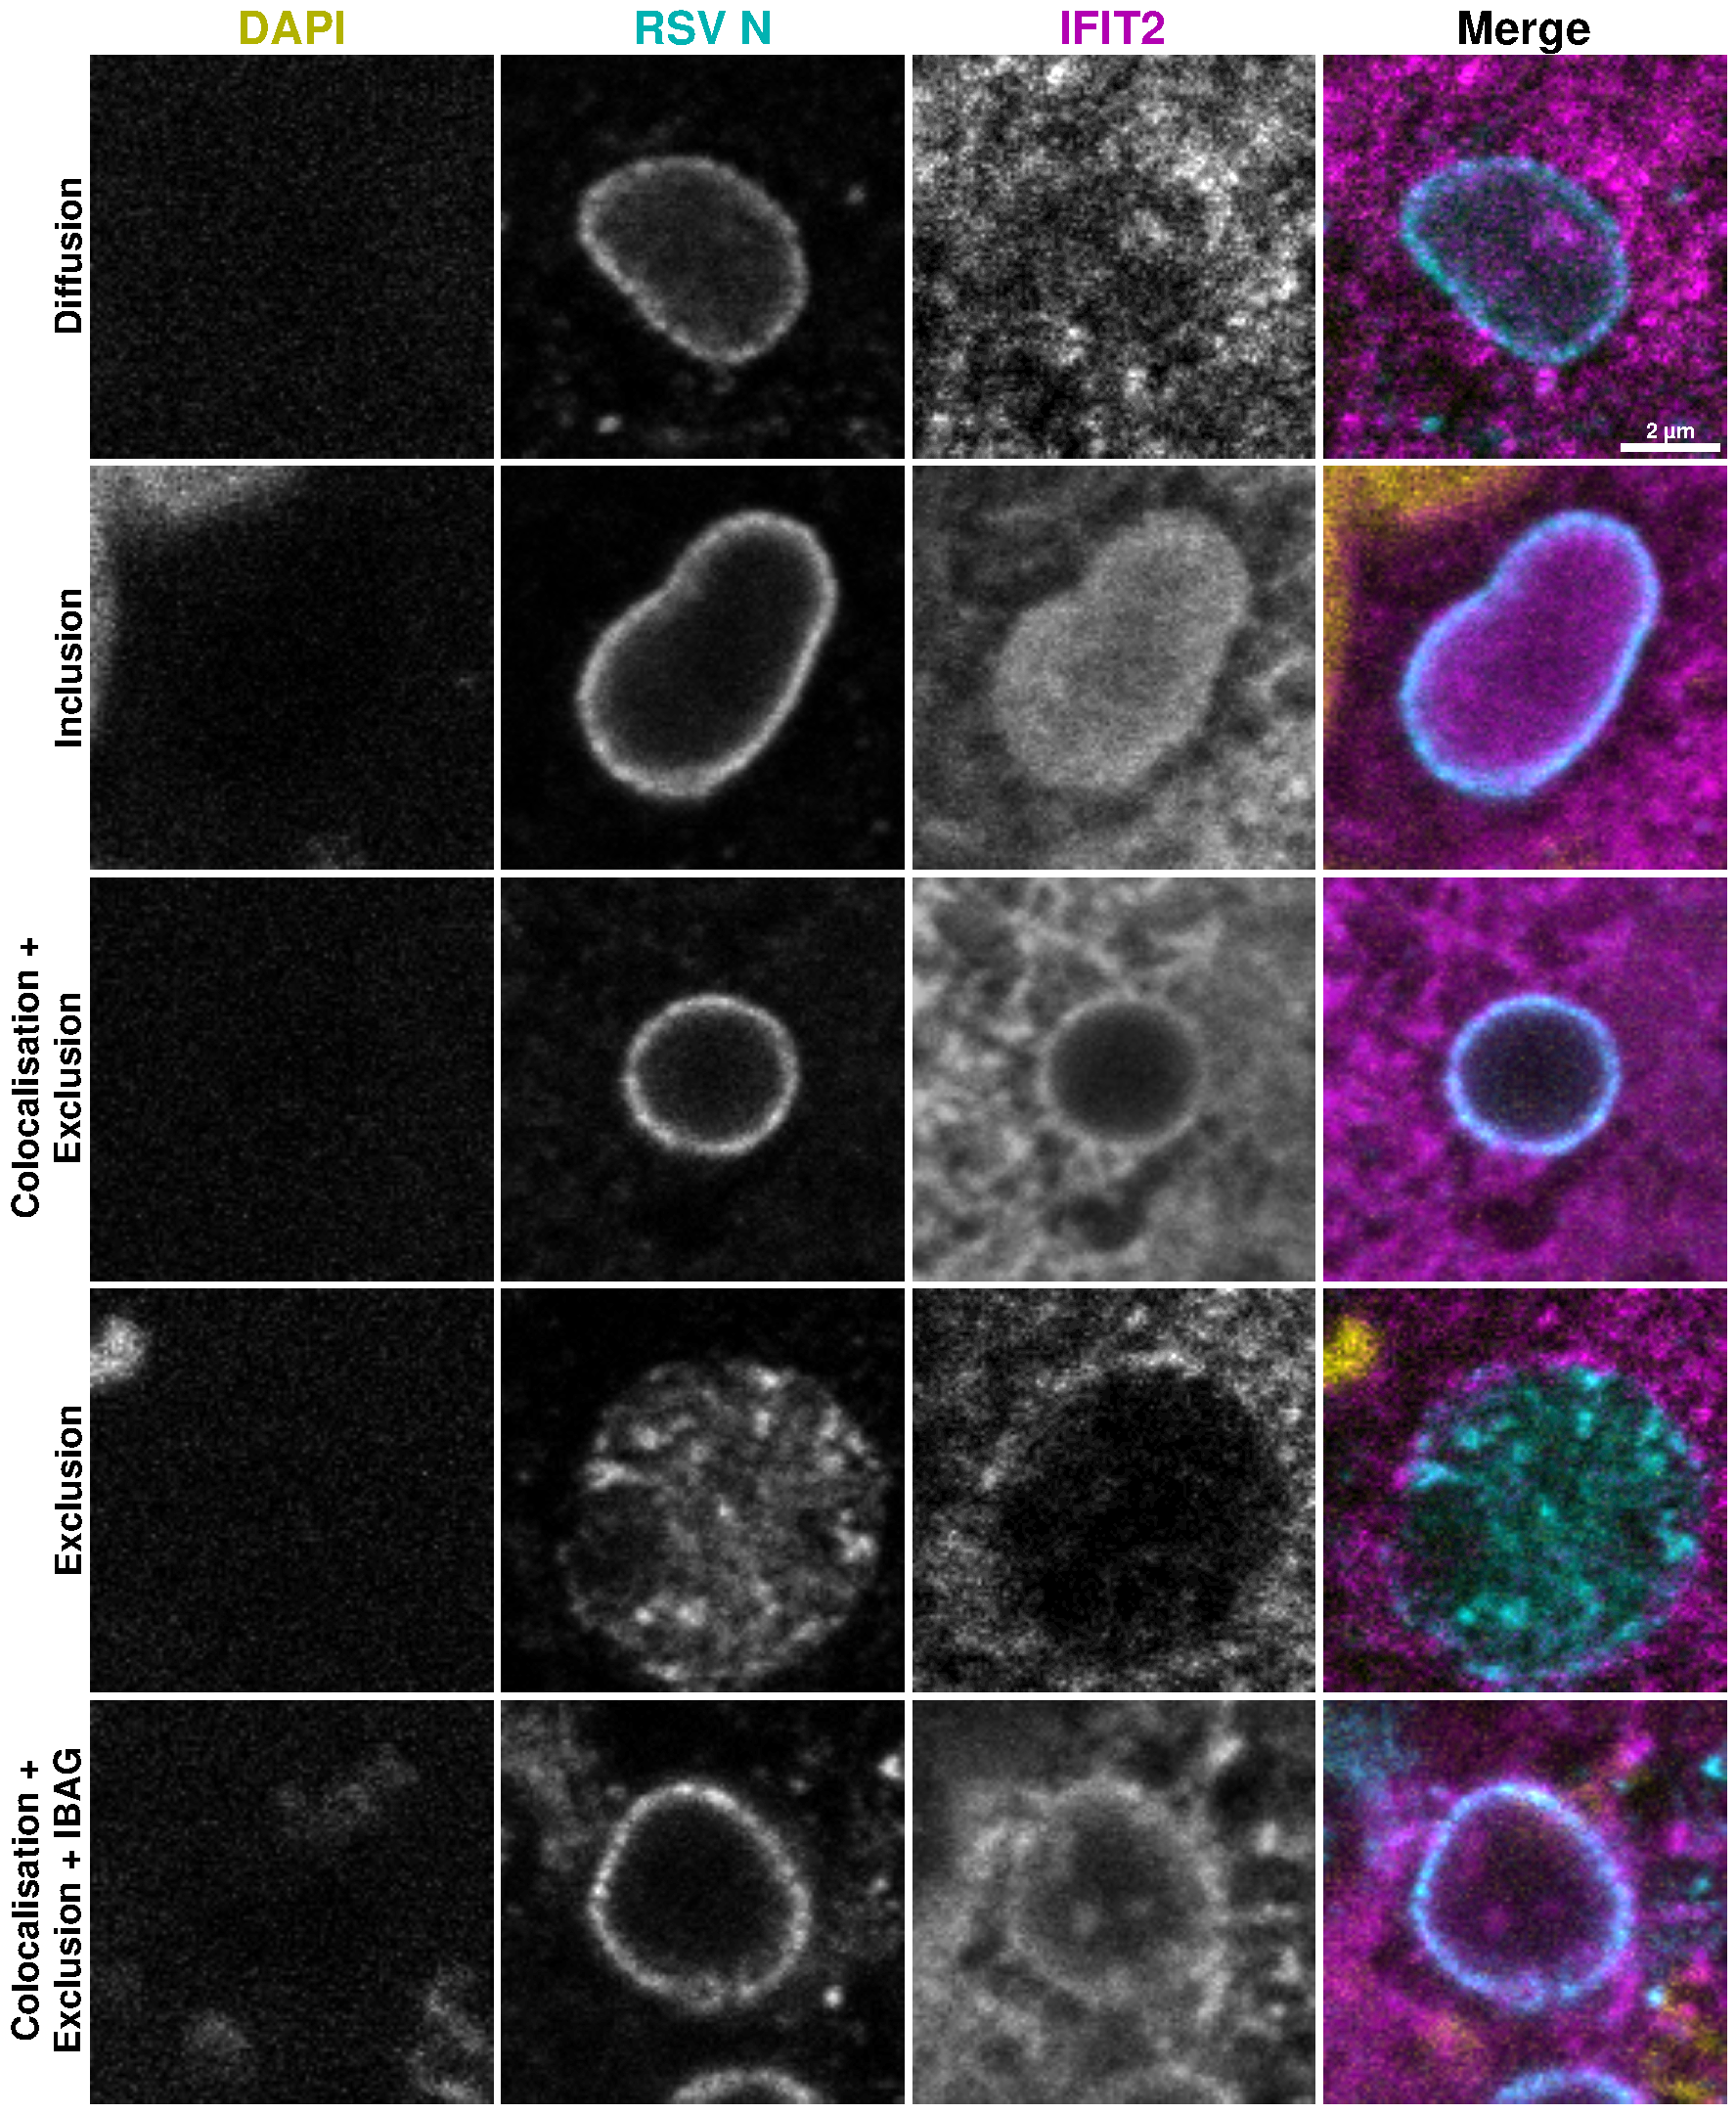
\includegraphics[width=1\linewidth]{09. Chapter 4/Figs/03. IFIT2-FLAG/03. IFIT2F/02. Infection Transfection/03. hi2f-hrsv.pdf}
    \caption[Representative Images of Observed Phenotypes of Exogenous hIFIT2 in the Context of hRSV Inclusion Bodies in VERO Cell Line.]{\textbf{Representative Images of Observed Phenotypes of Exogenous hIFIT2 in the Context of hRSV Inclusion Bodies in VERO Cell Line.} Vero cells were infected with human RSV at MOI 1. 24 HPI, the cells were transfected with hIFIT2-FLAG containing plasmids using TransIT-X2 and were fixed after further 24 hours. Cellular nuclei were stained with DAPI (yellow), and cells were double-labeled with anti-RSV N (cyan) and anti-FLAG (magenta) antibodies. This figure showcases representative examples of relevant phenotypes in the interaction between exogenous hIFIT2 and hRSV inclusion bodies. These phenotypes are presented in descending order based on their percentage proportions. The scale bar indicates 2 \(\mu m\).}
    \label{fig:Representative Images of Observed Phenotypes of Exogenous hIFIT2 in the Context of hRSV Inclusion Bodies in VERO Cell Line}
\end{figure}

In the follow up experiment, exogenous bovine IFIT2 in the context of human RSV infection shows the same two phenotypes. It is either excluded from the IBs (middle panel) or colocalises with the ring structure of the IBs (top and bottom panel; highlighted with arrows).

\begin{figure}
    \begin{subfigure}{0.495\textwidth}
        \caption{}
        \includegraphics[width=1\linewidth]{09. Chapter 4/Figs/03. IFIT2-FLAG/03. IFIT2F/02. Infection Transfection/04. bar_bi2f_hrsv.pdf} 
    \end{subfigure}
    \begin{subfigure}{0.495\textwidth}
        \caption{}
        \includegraphics[width=1\linewidth]{09. Chapter 4/Figs/03. IFIT2-FLAG/03. IFIT2F/02. Infection Transfection/05. box_bi2f_hrsv.pdf}
    \end{subfigure}
    \caption[Observed Phenotypes of Exogenous bIFIT2 in the Context of hRSV Inclusion Bodies in VERO Cell Line.]{\textbf{Observed Phenotypes of Exogenous bIFIT2 in the Context of hRSV Inclusion Bodies in VERO Cell Line.} Vero cells were infected with human RSV at MOI 1. 24 HPI, the cells were transfected with bIFIT2-FLAG containing plasmids using TransIT-X2 and were fixed after further 24 hours. Cells were labeled with anti-RSV N and anti-FLAG antibodies and imaged on confocal microscope. Panel (a) shows percentual proportions of observed phenotypes between hRSV inclusion bodies and exogenous bIFIT2 (62 observations), with the red dotted line denoting the 5\% threshold, marking phenotypes considered relevant above this limit. Panel (b) shows the IB area in \(\mu m^2\) per observed relevant phenotype.}
    \label{fig:Observed Phenotypes of Exogenous bIFIT2 in the Context of hRSV Inclusion Bodies in VERO Cell Line}
\end{figure}

\begin{figure}
    \centering
    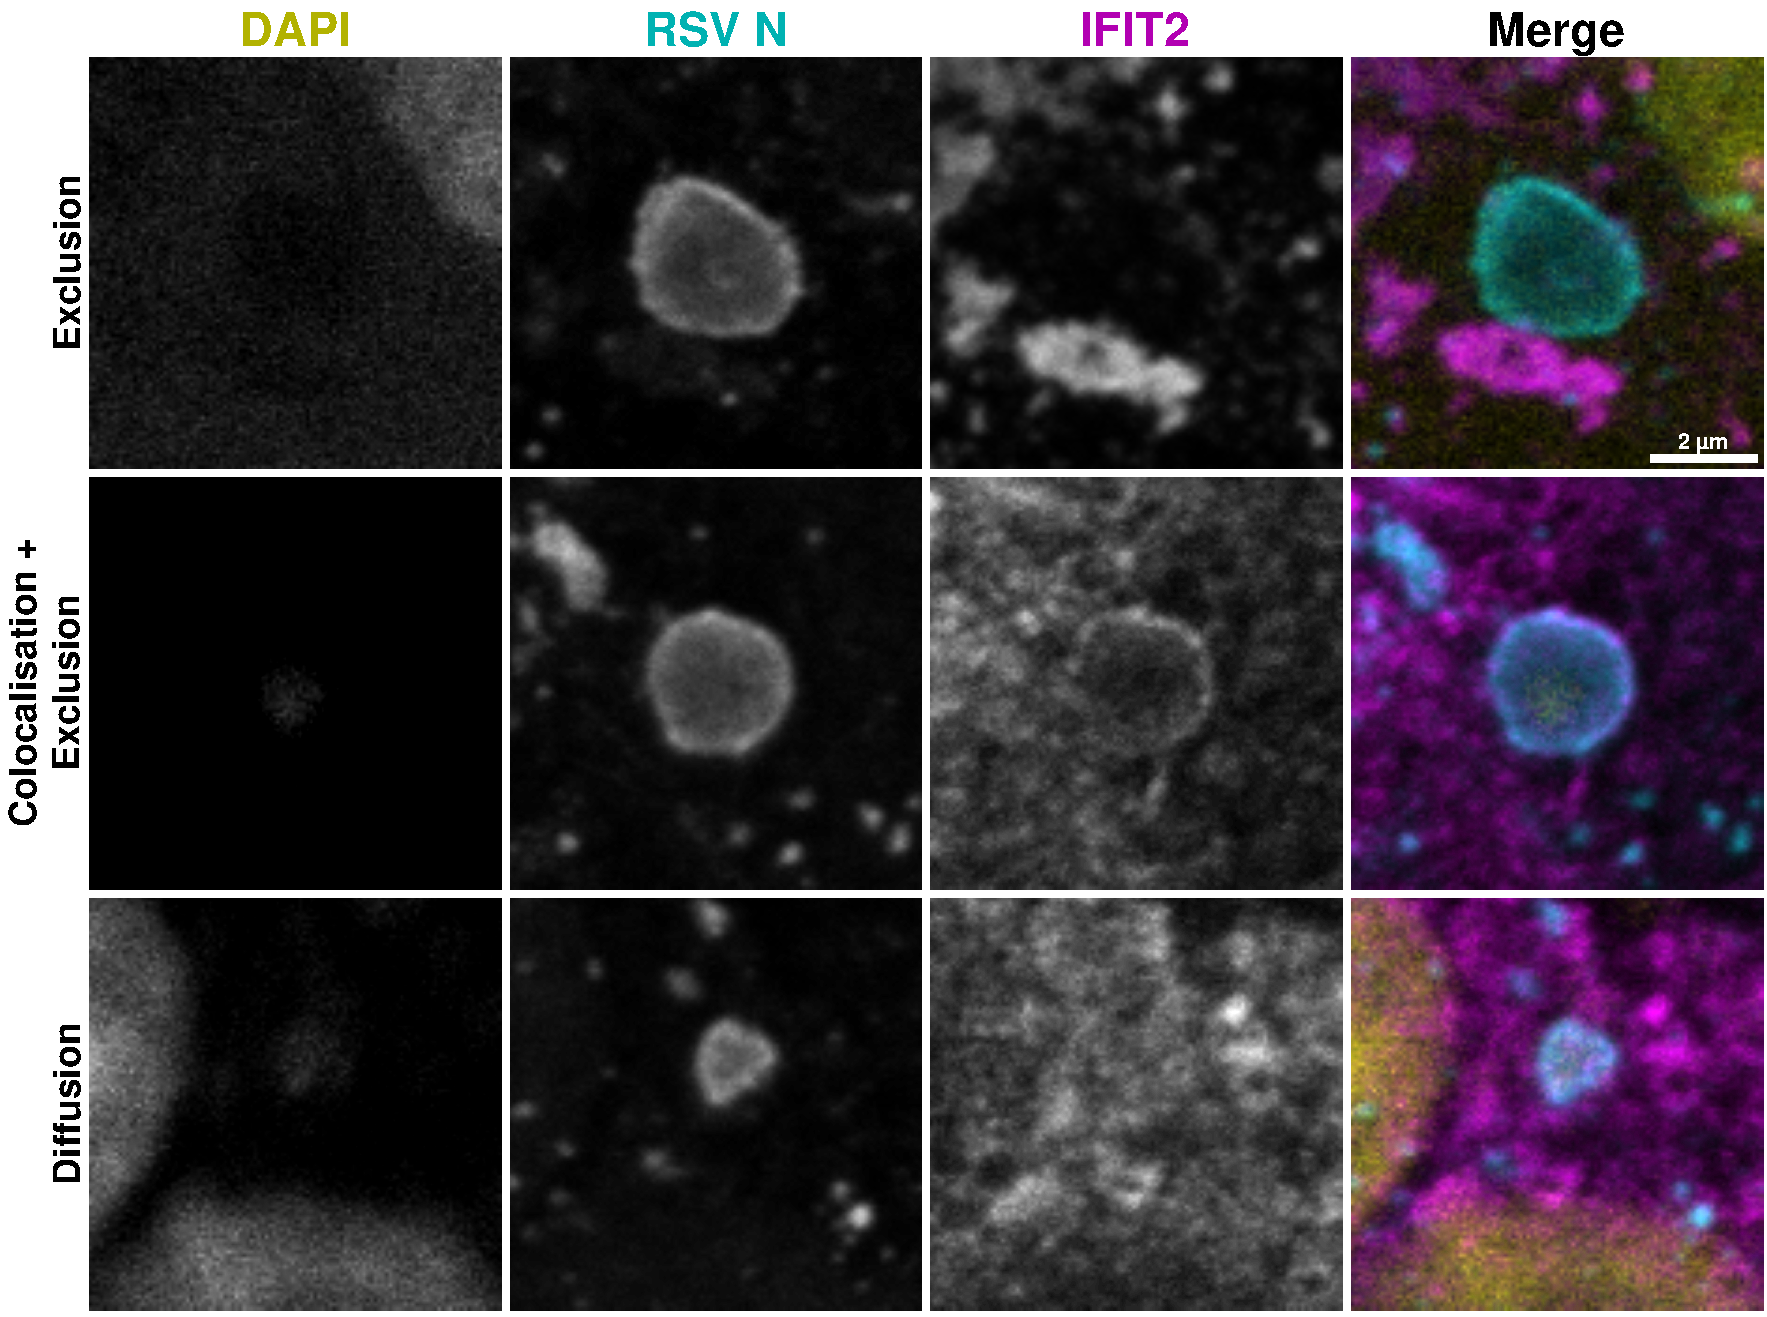
\includegraphics[width=1\linewidth]{09. Chapter 4/Figs/03. IFIT2-FLAG/03. IFIT2F/02. Infection Transfection/06. bi2f-hrsv.pdf}
    \caption[Representative Images of Observed Phenotypes of Exogenous bIFIT2 in the Context of hRSV Inclusion Bodies in VERO Cell Line.]{\textbf{Representative Images of Observed Phenotypes of Exogenous bIFIT2 in the Context of hRSV Inclusion Bodies in VERO Cell Line.} Vero cells were infected with human RSV at MOI 1. 24 HPI, the cells were transfected with bIFIT2-FLAG containing plasmids using TransIT-X2 and were fixed after further 24 hours. Cellular nuclei were stained with DAPI (yellow), and cells were double-labeled with anti-RSV N (cyan) and anti-FLAG (magenta) antibodies. This figure showcases representative examples of relevant phenotypes in the interaction between exogenous bIFIT2 and hRSV inclusion bodies. These phenotypes are presented in descending order based on their percentage proportions. The scale bar indicates 2 \(\mu m\).}
    \label{fig:Representative Images of Observed Phenotypes of Exogenous bIFIT2 in the Context of hRSV Inclusion Bodies in VERO Cell Line}
\end{figure}

Exogenous bovine IFIT2 during bovine RSV infection seems to be excluded from the inclusion bodies, although the data is not great and the IFIT2 is aggregated in both cells shown.

\begin{figure}
    \begin{subfigure}{0.495\textwidth}
        \caption{}
        \includegraphics[width=1\linewidth]{09. Chapter 4/Figs/03. IFIT2-FLAG/03. IFIT2F/02. Infection Transfection/07. bar_bi2f_brsv.pdf} 
    \end{subfigure}
    \begin{subfigure}{0.495\textwidth}
        \caption{}
        \includegraphics[width=1\linewidth]{09. Chapter 4/Figs/03. IFIT2-FLAG/03. IFIT2F/02. Infection Transfection/08. box_bi2f_brsv.pdf}
    \end{subfigure}
    \caption[Observed Phenotypes of Exogenous bIFIT2 in the Context of bRSV Inclusion Bodies in VERO Cell Line.]{\textbf{Observed Phenotypes of Exogenous bIFIT2 in the Context of bRSV Inclusion Bodies in VERO Cell Line.} Vero cells were infected with human RSV at MOI 1. 24 HPI, the cells were transfected with bIFIT2-FLAG containing plasmids using TransIT-X2 and were fixed after further 24 hours. Cells were labeled with anti-RSV N and anti-FLAG antibodies and imaged on confocal microscope. Panel (a) shows percentual proportions of observed phenotypes between bRSV inclusion bodies and exogenous bIFIT2 (31 observations), with the red dotted line denoting the 5\% threshold, marking phenotypes considered relevant above this limit. Panel (b) shows the IB area in \(\mu m^2\) per observed relevant phenotype.}
    \label{fig:Observed Phenotypes of Exogenous bIFIT2 in the Context of bRSV Inclusion Bodies in VERO Cell Line}
\end{figure}

\begin{figure}
    \centering
    \includegraphics[width=1\linewidth]{09. Chapter 4/Figs/03. IFIT2-FLAG/03. IFIT2F/02. Infection Transfection/09. bi2f-brsv.pdf}
    \caption[Representative Images of Observed Phenotypes of Exogenous bIFIT2 in the Context of bRSV Inclusion Bodies in VERO Cell Line.]{\textbf{Representative Images of Observed Phenotypes of Exogenous bIFIT2 in the Context of bRSV Inclusion Bodies in VERO Cell Line.} Vero cells were infected with human RSV at MOI 1. 24 HPI, the cells were transfected with bIFIT2-FLAG containing plasmids using TransIT-X2 and were fixed after further 24 hours. Cellular nuclei were stained with DAPI (yellow), and cells were double-labeled with anti-RSV N (cyan) and anti-FLAG (magenta) antibodies. This figure showcases representative examples of relevant phenotypes in the interaction between exogenous bIFIT2 and bRSV inclusion bodies. These phenotypes are presented in descending order based on their percentage proportions. The scale bar indicates 2 \(\mu m\).}
    \label{fig:Representative Images of Observed Phenotypes of Exogenous bIFIT2 in the Context of bRSV Inclusion Bodies in VERO Cell Line}
\end{figure}

\subsubsection{Summary} \label{Summary-i2-flag}
Overexpressing human IFIT2-FLAG does not seem to be detrimental to the cells. Exogenous human IFIT2 seems to form inclusions inside human pIB structures. It also colocalises with the pIB associated filamentous network. This data is consistent with IFIT2A antibody staining. IFIT2B staining showed inclusion inside pIB but failed to show the colocalization with the filamentous network. Exogenous bovine IFIT2 colocalises to the edge of human pIBs, which is in contrast to what we see with endogenous and exogenous human IFIT2 and its interaction with human pIBs. Exogenous human IFIT2 during human RSV infection showed different phenotypes in 2 different experiments. In the first experiment we observed it to: form inclusions inside the IB structure; be excluded from IB but colocalise to the IB ring; be excluded from the IB but colocalise to the ring and have spots inside the IB structure; or to be diffused through cytoplasm and IB equally. In the second experiment we observed it to be either completely excluded from the IBs or to colocalise with them. Exogenous bovine IFIT2 during human RSV infection was either completely excluded from the IB or was colocalised to the ring of the structure. This was consistently seen in both experiments conducted. Exogenous bovine IFIT2 during bovine RSV infection seems to be excluded from the IBs.